% This file is created on a Overleaf Template.
% Contact: Aditya Jain; Roll: 20111004; adityaj20@iitk.ac.in; Mob: 8770743694
\documentclass{article}
\usepackage{hyperref}
\usepackage{graphicx}
\usepackage{subcaption} 
\graphicspath{ {./images/} }

%----------------------------------------------------------------------------------------
%	PACKAGES AND OTHER DOCUMENT CONFIGURATIONS
%----------------------------------------------------------------------------------------

\usepackage{amsmath,amsfonts,stmaryrd,amssymb} % Math packages

\usepackage{enumerate} % Custom item numbers for enumerations

\usepackage[ruled]{algorithm2e} % Algorithms

\usepackage[framemethod=tikz]{mdframed} % Allows defining custom boxed/framed environments

\usepackage{listings} % File listings, with syntax highlighting
\lstset{
	basicstyle=\ttfamily, % Typeset listings in monospace font
}

%----------------------------------------------------------------------------------------
%	DOCUMENT MARGINS
%----------------------------------------------------------------------------------------

\usepackage{geometry} % Required for adjusting page dimensions and margins

\geometry{
	paper=a4paper, % Paper size, change to letterpaper for US letter size
	top=2.5cm, % Top margin
	bottom=3cm, % Bottom margin
	left=2.5cm, % Left margin
	right=2.5cm, % Right margin
	headheight=14pt, % Header height
	footskip=1.5cm, % Space from the bottom margin to the baseline of the footer
	headsep=1.2cm, % Space from the top margin to the baseline of the header
	%showframe, % Uncomment to show how the type block is set on the page
}

%----------------------------------------------------------------------------------------
%	FONTS
%----------------------------------------------------------------------------------------

\usepackage[utf8]{inputenc} % Required for inputting international characters
\usepackage[T1]{fontenc} % Output font encoding for international characters

\usepackage{XCharter} % Use the XCharter fonts

%----------------------------------------------------------------------------------------
%	COMMAND LINE ENVIRONMENT
%----------------------------------------------------------------------------------------

% Usage:
% \begin{commandline}
%	\begin{verbatim}
%		$ ls
%		
%		Applications	Desktop	...
%	\end{verbatim}
% \end{commandline}

\mdfdefinestyle{commandline}{
	leftmargin=10pt,
	rightmargin=10pt,
	innerleftmargin=15pt,
	middlelinecolor=black!50!white,
	middlelinewidth=2pt,
	frametitlerule=false,
	backgroundcolor=black!5!white,
	frametitle={Command Line},
	frametitlefont={\normalfont\sffamily\color{white}\hspace{-1em}},
	frametitlebackgroundcolor=black!50!white,
	nobreak,
}

% Define a custom environment for command-line snapshots
\newenvironment{commandline}{
	\medskip
	\begin{mdframed}[style=commandline]
}{
	\end{mdframed}
	\medskip
}

%----------------------------------------------------------------------------------------
%	FILE CONTENTS ENVIRONMENT
%----------------------------------------------------------------------------------------

% Usage:
% \begin{file}[optional filename, defaults to "File"]
%	File contents, for example, with a listings environment
% \end{file}

\mdfdefinestyle{file}{
	innertopmargin=1.6\baselineskip,
	innerbottommargin=0.8\baselineskip,
	topline=false, bottomline=false,
	leftline=false, rightline=false,
	leftmargin=2cm,
	rightmargin=2cm,
	singleextra={%
		\draw[fill=black!10!white](P)++(0,-1.2em)rectangle(P-|O);
		\node[anchor=north west]
		at(P-|O){\ttfamily\mdfilename};
		%
		\def\l{3em}
		\draw(O-|P)++(-\l,0)--++(\l,\l)--(P)--(P-|O)--(O)--cycle;
		\draw(O-|P)++(-\l,0)--++(0,\l)--++(\l,0);
	},
	nobreak,
}

% Define a custom environment for file contents
\newenvironment{file}[1][File]{ % Set the default filename to "File"
	\medskip
	\newcommand{\mdfilename}{#1}
	\begin{mdframed}[style=file]
}{
	\end{mdframed}
	\medskip
}

%----------------------------------------------------------------------------------------
%	NUMBERED QUESTIONS ENVIRONMENT
%----------------------------------------------------------------------------------------

% Usage:
% \begin{question}[optional title]
%	Question contents
% \end{question}

\mdfdefinestyle{question}{
	innertopmargin=1.2\baselineskip,
	innerbottommargin=0.8\baselineskip,
	roundcorner=5pt,
	nobreak,
	singleextra={%
		\draw(P-|O)node[xshift=1em,anchor=west,fill=white,draw,rounded corners=5pt]{%
		Question \theQuestion\questionTitle};
	},
}

\newcounter{Question} % Stores the current question number that gets iterated with each new question

% Define a custom environment for numbered questions
\newenvironment{question}[1][\unskip]{
	\bigskip
	\stepcounter{Question}
	\newcommand{\questionTitle}{~#1}
	\begin{mdframed}[style=question]
}{
	\end{mdframed}
	\medskip
}

%----------------------------------------------------------------------------------------
%	WARNING TEXT ENVIRONMENT
%----------------------------------------------------------------------------------------

% Usage:
% \begin{warn}[optional title, defaults to "Warning:"]
%	Contents
% \end{warn}

\mdfdefinestyle{warning}{
	topline=false, bottomline=false,
	leftline=false, rightline=false,
	nobreak,
	singleextra={%
		\draw(P-|O)++(-0.5em,0)node(tmp1){};
		\draw(P-|O)++(0.5em,0)node(tmp2){};
		\fill[black,rotate around={45:(P-|O)}](tmp1)rectangle(tmp2);
		\node at(P-|O){\color{white}\scriptsize\bf !};
		\draw[very thick](P-|O)++(0,-1em)--(O);%--(O-|P);
	}
}

% Define a custom environment for warning text
\newenvironment{warn}[1][Warning:]{ % Set the default warning to "Warning:"
	\medskip
	\begin{mdframed}[style=warning]
		\noindent{\textbf{#1}}
}{
	\end{mdframed}
}

%----------------------------------------------------------------------------------------
%	INFORMATION ENVIRONMENT
%----------------------------------------------------------------------------------------

% Usage:
% \begin{info}[optional title, defaults to "Info:"]
% 	contents
% 	\end{info}

\mdfdefinestyle{info}{%
	topline=false, bottomline=false,
	leftline=false, rightline=false,
	nobreak,
	singleextra={%
		\fill[black](P-|O)circle[radius=0.4em];
		\node at(P-|O){\color{white}\scriptsize\bf i};
		\draw[very thick](P-|O)++(0,-0.8em)--(O);%--(O-|P);
	}
}

% Define a custom environment for information
\newenvironment{info}[1][Info:]{ % Set the default title to "Info:"
	\medskip
	\begin{mdframed}[style=info]
		\noindent{\textbf{#1}}
}{
	\end{mdframed}
}




%----------------------------------------------------------------------------------------
%	ASSIGNMENT INFORMATION
%----------------------------------------------------------------------------------------

\title{CS85A: Data Mining Assignment \#1 } % Title of the assignment

\author{Aditya Jain\\ 20111004   \\\texttt{adityaj20@iitk.ac.in}} % Author name and email address

\date{Indian Institute of Technology, Kanpur--- \today} % University, school and/or department name(s) and a date

%----------------------------------------------------------------------------------------

\begin{document}

\maketitle % Print the title

%----------------------------------------------------------------------------------------
%	INTRODUCTION
%----------------------------------------------------------------------------------------

\section{Introduction} % Unnumbered section

India is facing an unprecedented crisis due to the novel coronavirus, first reported in Wuhan, China in December 2019. In India COVID was first reported on January 30, 2020, in Kerala and it upsurged very quickly to all states in the country. The total number of confirmed cases are more than 54 Lakhs to date (September 20, 2020). It has disrupted the lives of 1.3 billion Indians, first with a complete lockdown in the country from March 24 - May 31, 2020, then various aspects as work from home, etc.\\\\

In this project, I have tried to analyse the growth of cases in each district for every week, month and overall from \textbf{March 15 - September 5, 2020.} There were total of 112 cases before March 15 and 41,10,839 on September 5, 2020. Districts are classed as hotspot and coldspot per week, month, and overall concerning their neighbours and in overall state.  

\subsection{Data collection}

Data for this study is collected from covid19india.org. Following csv files are incorporated for data processing to generate the results: 
\begin{enumerate}
    \item \href{https://api.covid19india.org/csv/latest/raw\_data1.csv}{raw\_data1.csv} - It contains patient wise data till April 19.
    \item \href{https://api.covid19india.org/csv/latest/raw\_data2.csv}{raw\_data2.csv} - It contains patient wise data from April 20 to April 26.
    \item districts.csv - District wise timeseries of Confirmed, Recovered and Deceased numbers from April 26 to Sep 6 2020.
    \item neighbor-districts-modified.json - List of neighbours of each district of India
\end{enumerate}

\subsection{Data Pre-processing}
\begin{itemize}
    \item Due to errors in district-wise data of state Assam, Telangana, Goa, Delhi and city Mumbai I have merged all their districts as one single district.
    \item Cases of districts that didn't map to the neighbour-district file and the ones titled as "Unknown" are removed from the dataset.
  
\end{itemize}

A total of 41,10,839 cases are recorded in the input files from covid19.org for the period March 15 to September 5, 2020. After complete processing total of 40,50,336 cases for 645 different districts are obtained. 




%----------------------------------------------------------------------------------------
%	OBSERVATION
%----------------------------------------------------------------------------------------
\pagebreak
\section{Observations} % Numbered section

%------------------------------------------------
\subsection{Total Cases as of Sep 5, 2020}
Following graph shows the total number of confirmed COVID cases for each district in India.\\
\begin{figure}[h]
    \centering
    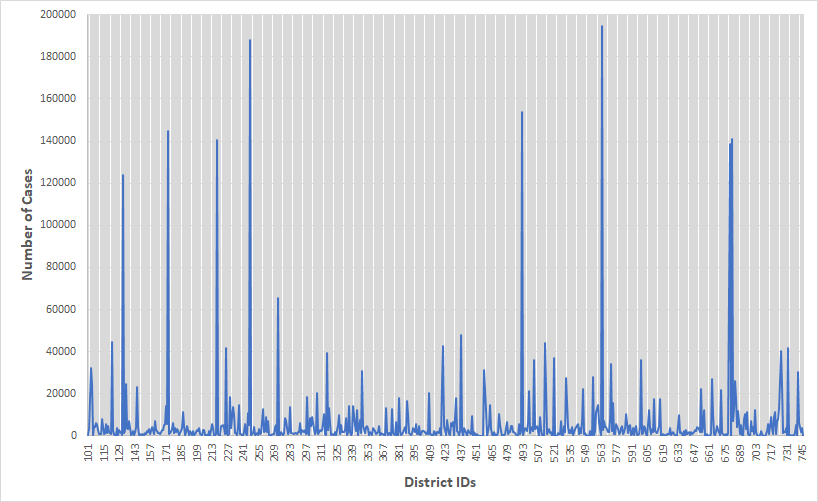
\includegraphics[scale = 0.76]{images/cases-districtid.png}
    \caption{Total recorded cases for each district.}
\end{figure}

\begin{itemize}
    \item There are nine districts with more than 1 lakh cases in which Pune, Delhi, Mumbai and Bengaluru are on top. 
   \item There are 17 districts more than 30 thousand cases.
   \item Rest 619 districts have fewer cases.
\end{itemize}
These results show that major cases are restricted to some districts rather than equal distribution. I haven't included population per capita statistics in our analysis which may be the reason our results are showing some highly populated districts as hotspots. 

%------------------------------------------------
\subsection{COVID-19 entrance in India}
The COVID-19 cases appeared in March 2020 were related to people who have been evacuated or have arrived from COVID-19–affected countries. There were  632 such foreign cases out of 1013 total cases to date March 23, 2020, from which government suspended international travel till July 31, 2020.

\begin{figure}[h]
    \centering
    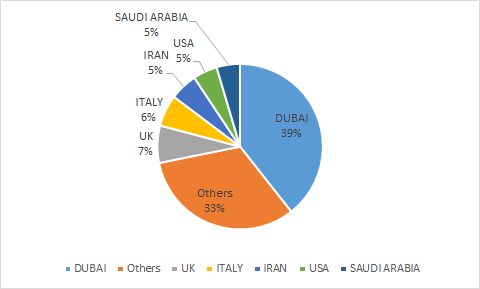
\includegraphics{Fig1}
    \caption{Cases arrived from foreign countries before international travel ban.}
\end{figure}
\pagebreak

Travellers from Italy, Dubai, US, and the UK comprise 61\% of these cases, and Kerala was the most affected by these foreign cases with a count of 221.\\ 28 out of 36 states have recorded at least a case with foreign travel history. These foreign cases were the start of the pandemic in the country. 


	
%------------------------------------------------

\subsection{Month-wise spread}

\begin{figure}[h]
    \centering
    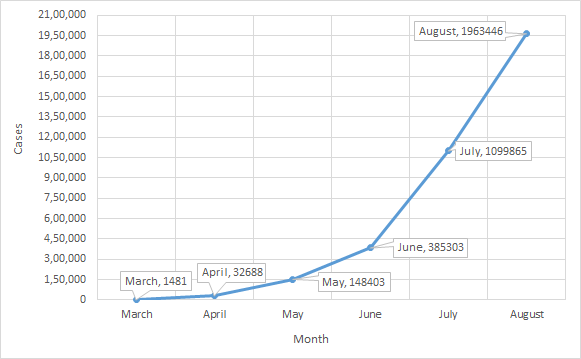
\includegraphics{MonthvsCases}
    \caption{Curve representing number of new cases generated every month }
\end{figure}
The number of new cases reported each month is approximately 2.39 times the cases generated in the previous month except for April. The number of new cases in April was 4.5 times the number reported in March. So data suggests that:
\begin{itemize}
    \item India was in stage 1 (disease through people with travel history) of COVID-19 in March with only 169 affected districts. 
    \item Stage 2 (local transmission - friends and family of people with travel history) started in April with 422 affected districts.
    \item Stage 3 (community transmission - when the source for the virus cannot be traced) started in May with 592 affected districts.
   \item 641 districts out of 645 districts had reported a case of COVID-19 till June 2020. All 645 districts were affected by August, 2020.
\end{itemize}

%------------------------------------------------
\subsection{Week-wise spread}

\begin{figure}[h]
    \centering
    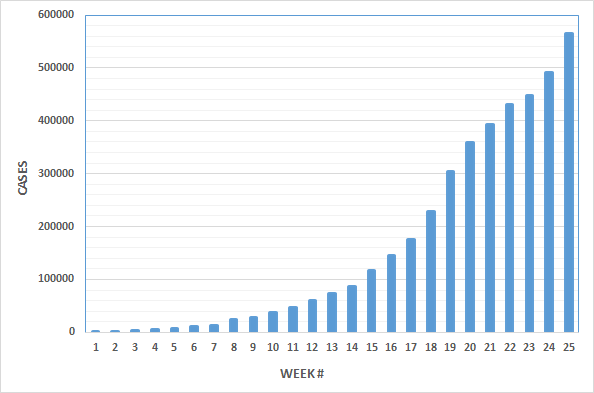
\includegraphics[scale=0.7]{WeekvsCases}
    \caption{Cases spread over the weeks}
\end{figure}

I have discretized the data set into weeks such that March 15 - March 21, 2020, is week 1 and so on. Above graph represents the number of new cases reported each week from March 15 to September 5, 2020. Graph shows exponential growth in cases over weeks.
\subsection{Hotspots Analysis}
\subsubsection{Hotspot among neighbouring districts}
I have categorized the districts into a hotspot if the number of cases recorded in the districts is greater than the sum of the mean and standard deviation of its neighbour districts cases. Following is the graph showing number of hotspot districts in each month:
\begin{figure}[h]
    \centering
    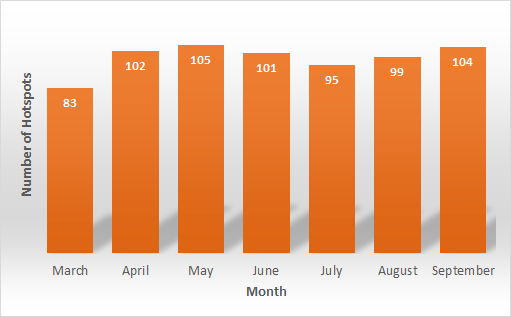
\includegraphics{images/neighbour-month-hotspots.png}
    \caption{Number of hotspot districts among their neighbors over months}
\end{figure}
\\
A district is hotspot if the difference between the number of cases incurred in it is very large than the cases incurred in its neighbouring districts. Analysis shows that on an average a district remains a hotspot for around 3-4 months only. There are only 21 such districts which remained hotspots for all seven months of the analysis. This means that once a district becomes a hotspot, there is an increase in growth rate of COVID cases in its neighbouring districts, reducing the difference between the number of cases in hotspot and its neighbouring districts.\\
So we can speculate that the infection spreads from a hotspot district to its neighbours within a month period, as very few districts remain hotspots among its niehgbours as we move across the timeline.

\subsubsection{Hotspot within a State}
I have categorized the districts into a hotspot if the number of cases recorded in the districts is greater than the sum of the mean and standard deviation of its state districts cases. Following is the graph showing number of hotspot districts in each month:
\begin{figure}[h]
    \centering
    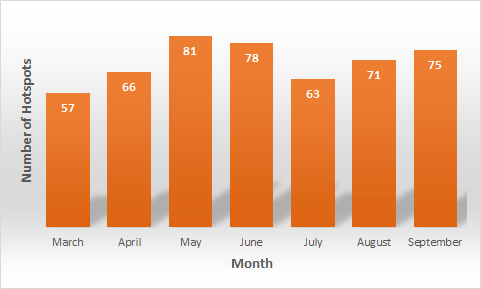
\includegraphics{images/state-month-hotspots.png}
    \caption{Number of State hotspot districts}
\end{figure}
\\
Since there was a significant hike in the number of hotspots in May, it shows that in May and June most cases were restricted to the main hub cities of the state. This conclusion is also backed by the fact that inter-district travel was highly restricted due to nation-wide lockdown placed by the government until June 2020. Till July most districts of the state started recording significant cases, and hence the number of hotspots get normalized to normal range from July. \\
Analysis shows that only 18 districts remained hotspots in all the months, so we may conclude that virus migrated in large numbers from these hubs to other districts of the state in July when the lockdown was also removed.
\subsection{Coldspots Analysis}
I have categorized the districts into a coldspot if the number of cases recorded in the districts is smaller than the subtraction of the mean and standard deviation of its neighbour districts (for neighbour analysis) and state districts (for state analysis) cases. Following is the graph showing number of coldspots districts in each month for both the ases:
\begin{figure}[!h] 
    \centering
	\begin{subfigure}[b]{7cm} 
		\centering 
		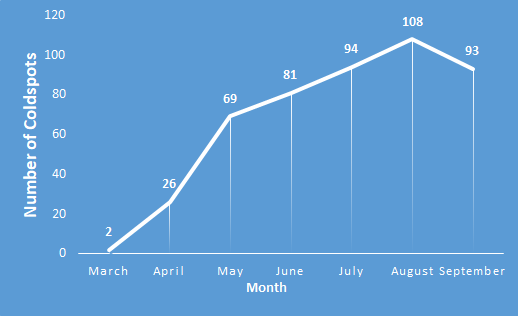
\includegraphics[scale=0.74]{images/neighbour-month-coldspots.png}
		\caption{Number of State coldspot districts} 
	\end{subfigure} 
	\hspace{0cm} 
	\begin{subfigure}[b]{8cm} 
		\centering 
		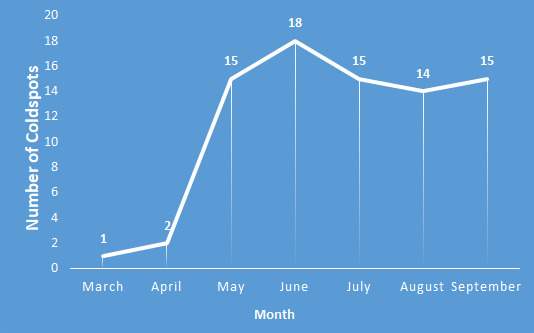
\includegraphics[scale=0.7]{images/sate-month-coldspots.png}
		\caption{Number of coldspot districts among their neighbors} 
	\end{subfigure} 
\end{figure}
\\
We observed that the number of coldspots have increased every month for both the cases (State and Neigbour analysis). This increase of coldspots also shows that a large number of patients are restricted to some districts. Cases are rising at a tremendous rate in these hubs with respect to the other districts in the state, making their neighbours classify as coldspots. These hubs are the districts with a large population per capita density. 
\\
The number of coldspots will keep on increasing to a point and then will gradually fall when the majority of the population in these hubs are recovered from the disease.

%------------------------------------------------
\section{Conclusion}
COVID cases in India are rising day by day and don't seem to stall as the infection has just penetrated 0.3\% of the population. A large number of cases are restricted to some districts only their growth rate is tremendious as compared to the districts around them. \\
\\
We saw that number of hotspots are constant among the months, and the number of coldspots is increasing every month. This pattern will follow due to different population per capita in different districts.


%----------------------------------------------------------------------------------------

\end{document}
